\chapter{Results exploitation}

\begin{summary}
\lipsum[1]
\end{summary}

\section{Introduction}
In Chapter \ref{cha:model} we have shown how a 3D-SIC can be modelled and the problem we are dealing with in this work, as well as simulation results based on multi-objective optimization. In Chapter \ref{cha:robustness}, we have shown that the methodology can show good convergence and diversity properties even if the problem contains criteria of heterogeneous nature. In this Chapter, we will discuss about how a designer could use these results and take advantage of a multi-criteria oriented methodology in the process of producing a 3D-SIC to, for instance, make a choice among the solutions of the Pareto frontier.

\section{Preference modelling}
As explained in Chapter \ref{cha:rol.mcda}, once a Pareto front has been determined or approximated, the next step is to choose among this set of solutions. One way to help decision makers to make their choice is to model their preferences, for instance with an outranking method. In the scope of this work, we will present the use of the PROMETHEE methodology as it has been developed in our department and has also shown good results in different fields \cite{Beh2010}.

\subsection{Using the PROMETHEE methods}

\subsubsection{Building a PROMETHEE model}
In order to use the PROMETHEE method, the decision maker has to inform about his preferences on the criteria, these being preference functions, indifference and preference thresholds and weights on the criteria (see Chapter \ref{cha:rol.mcda}). To illustrate this, we will use a PROMETHEE software called D-Sight that has been developed by Quantin Hayez and use the results of the simulations presented in Chapter \ref{cha:robustness}. In those results, there are 804 alternatives in the Pareto front, evaluated on 5 criteria. The evaluation table can be found in Appendix \ref{}. Let us take a simple example of preference modelling in order to illustrate what kind of aid a multi-criteria analysis can provide.

First, we have to define preference functions for each criterion. For the interconnection distance, cost, volume and clock position, we will choose a V-shape function. With this function, the preference index will increase linearly until a preference threshold is reached which can be the case for these criteria. For the power dissipation, we will choose a U-shape function where there is no preference until an indifference threshold is reached. Indeed there can be no real problem if the difference between two circuits in terms of heat dissipation is low, and it can be directly problematic when this difference is high.

The thresholds will be set at a difference of 10\% in the evaluations. For the weights, we will consider that the interconnection distance, the cost and the power dissipation are more important than the volume and the clock position, with the volume less important than the clock position. We will choose arbitrarily the weights and also suppose that the three first cited criteria share the same importance (25\% each) and two remaining ones taking the last 25\% (14\% and 11\% respectively). Let us note that it is possible to elicit the weights by answering simple questions, for instance with AHP.

A summary of all these data is given in Table \ref{tab:preffunc}. Of course, a more accurate model could be defined, however let us remind that the purpose here is to show how a multi-criteria analysis can give added information to designers.

\begin{table}[h!]
\caption{PROMETHEE model}
\begin{center}
\begin{tabular}{|c|c|c|c|c|}
\hline
Criterion & Preference & Indifference  & Preference & Weight \\
 & function & threshold & threshold & \\
\hline
Interconnection distance & V-shape & x & 10\% & 25\% \\
Cost & V-shape & x & 10\% & 25\% \\
Volume & V-shape & x & 10\% & 11\% \\
Clock position & V-shape & x & 10\% & 14\% \\
Power dissipation & U-shape & 10\% & x & 25\% \\
\hline
\end{tabular}
\end{center}
\label{tab:preffunc}
\end{table}

Now that a model has been proposed, let us analyse the results produced by D-Sight.

\subsubsection{Multi-criteria analysis}

\paragraph{PROMETHEE rankings}
D-Sight will do all the computations of the flows and PROMETHEE (I and II) rankings can be obtained, based on the preferences. A decision maker can make a choice based on these rankings, for example by choosing the solution ranked first. In addition, other tools are available, that allow to have a transparent decision process and analyse the set of solutions to know why a given ranking is obtained. One of the most useful one is the GAIA plane which is illustrated in Figure \ref{fig:gva804} (for the sake of readability, the alternatives' name has been removed).

\begin{figure}[h!]
\begin{center}
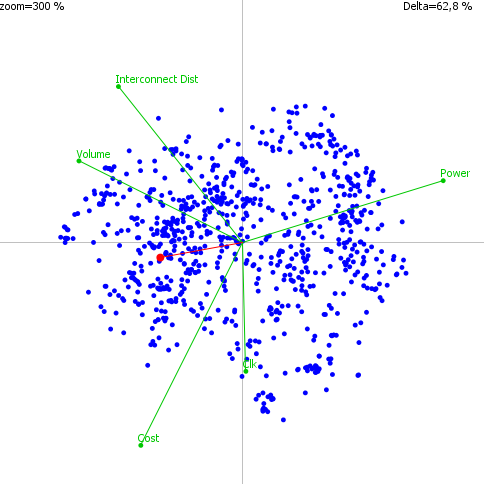
\includegraphics[width=0.8\linewidth]{gva804}
\end{center}
\caption{GAIA plane of the case study}
\label{fig:gva804}
\end{figure}

As a reminder from Chapter \ref{cha:rol.mcda}, the GAIA plane is based on the principal component analysis of the unicriterion net flows of the solutions and minimises the projection error of each alternative on it. Four distinctive visual information are shown:
\begin{enumerate}
\item The green axes that represent the projections of each criterion's axis.
\item The blue dots that represent the projection of each solution's uni-criterion net flow. The value of the uni-criterion net flow is read by projecting the point on the related criterion axis.
\item The red axis that represents the \textit{decision stick} which is the projection of the set of weights and gives the decision direction.
\item The \textit{delta} value that represents the percentage of kept information since there are projection errors.
\end{enumerate}

The first observation that can be drawn is that the blue dots are at the same time well-spread and dense, which illustrate the conclusions of Chapter \ref{cha:robustness}. This also means that each criterion is well-represented in terms of solutions.

Second, let us take a look at the information that is provided by the criteria axes (green). This is shown in Figure \ref{fig:gva804crit}.

\begin{figure}[h!]
\begin{center}
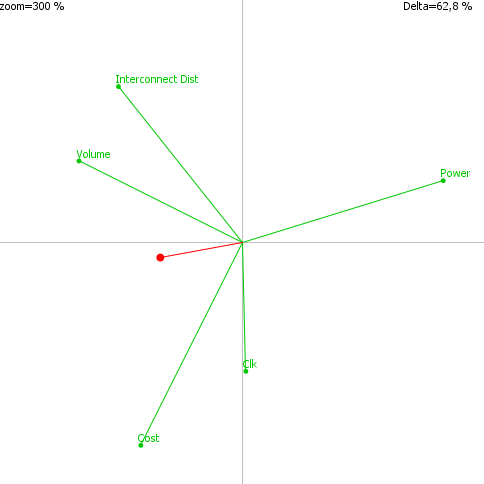
\includegraphics[width=0.8\linewidth]{gva804crit}
\end{center}
\caption{GAIA plane of the case study (criteria axis only)}
\label{fig:gva804crit}
\end{figure}

From the GAIA plane, we can observe how the criteria are related between each other. Indeed, criteria axes that have opposite directions are conflicting, whereas criteria with the same direction share the same optimisation trend. In the present case, we can see that the criteria of interconnection distance, power dissipation and cost are conflicting, which reflects the design reality. Also, the volume criterion shares the same direction as the interconnection distance criterion which is normal as reducing the interconnection distance will also tend to reduce the circuit volume. These observations also confirm that the defined model is indeed consistent with the reality.

Finally, let us have a view at the information provided by the decision stick. As explained previously, the decision stick represent the criteria weights and therefore gives the decision direction. Indeed, the alternatives with the highest net flow score will have their furthest projection on that axis, in the direction of that axis (see Figure \ref{fig:gva804stick}). This visually represents the PROMETHEE II ranking,  provided that the \textit{delta} value shows that enough information has been kept with the projection. In this case, this value is relatively low (62.8\%) which means that a lot of information has been lost with the projection, that can lead, for instance, to PROMETHEE II ranking errors with the visual projections compared to the ranking obtained with the computed net flows.

\begin{figure}[h!]
\begin{center}
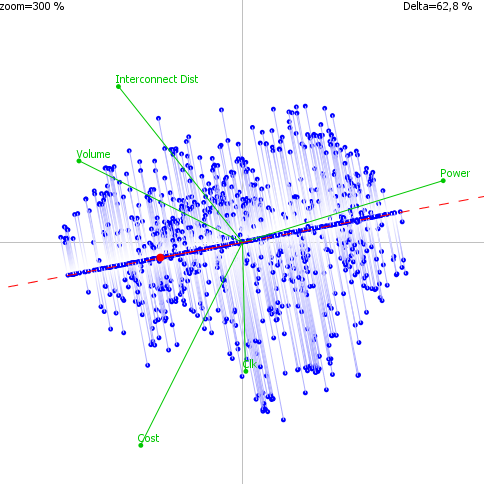
\includegraphics[width=0.8\linewidth]{gva804stick}
\end{center}
\caption{GAIA plane of the case study (with decision stick projection)}
\label{fig:gva804stick}
\end{figure}

\paragraph{Robustness analysis with stability intervals}
Another tool that can help decision makers is the robustness analysis that will allow them to know how stable a solution is, given the provided preference model. It is based on stability intervals on the weights where the first-ranked alternative will not change. This tool can be useful as there can be uncertainties on the values given for the weights. For the considered model, the stability intervals are shown in Table \ref{tab:stability}. We can observe that the first-ranked solution is relatively robust with all the criteria weights spanning on rather large intervals. This means that small uncertainties will not affect the ranking of the first alternative.

\begin{table}[h!]
\caption{Stability intervals (level 1)}
\begin{center}
\begin{tabular}{|c|c|c|c|}
\hline
Criterion & Min weight & Value  & Max weight \\
\hline
Interconnection distance & 5.73\% & 25\% & 50.00\% \\
Cost & 3.37\% & 25\% & 36.38\% \\
Volume & 0.00\% & 11\% & 23.85\% \\
Clock position & 2.06\% & 14\% & 43.06\% \\
Power dissipation & 17.85\% & 25\% & 68.21\% \\
\hline
\end{tabular}
\end{center}
\label{tab:stability}
\end{table}

\section{Constraint modelling}
Another way to help decision makers is to model constraints in order to eliminate unnecessary alternatives and reduce the number of solutions. For that purpose, we have developed a visual interface where a decision maker can introduce constraints to be fulfilled and see directly the remaining solutions.

\section{How to pertinently represent multi-criteria information}


\section{On the use of a multi-criteria paradigm in microelectronics design}
As described in Chapter \ref{cha:rol.icdesign}, the multi-criteria paradigm is rarely used in the field of IC design; at best, trade-off analyses are performed. To our knowledge, more global multi-criteria analyses have not been carried out yet.

When discussing with design experts, it is quite interesting to see how they easily understand the stake of the MCDA paradigm and how it would be able to help designers facing IC development challenges. However, it is more difficult to make them adopt this approach for three main reasons that have appeared throughout several discussions:

\begin{enumerate}
\item "It is not how we optimise circuits" seems to be one of the most frequent statements. Indeed, the industry follows a uni-criterion paradigm and is not used to first explore several possible solutions and then determine good compromise solutions. The designers will generally decide about an architecture and try to optimise it to achieve the specifications.
\item Designers can understand how preference modelling work, however they are not used to answer questions about indifference/preference thresholds or criteria weights as they receive specifications to achieve. This would need a change in how the design of a circuit is approached and how specifications are formulated.
\item As a consequence of the fact that design space exploration is based on performance assessment, preference modelling would be based on estimated metrics. While it will provide relevant ordered information, this will not necessarily match the values of real specifications. Therefore, this adds a level of difficulty for the modelling.
\end{enumerate}



\section{Conclusion}